% !TEX root = pfe-book2.tex
%!TEX TS-program = pdflatex
%!TEX encoding = UTF-8 Unicode


\cleardoublepage
%\mainmatter
\chapter{Molecular Mechanics}
\label{ch-06}

\section{Frictional Forces}

This isn’t the first time that we are speaking of fric­tion. And as a matter of fact, in telling about motion, how could we have managed without mentioning friction? Almost any motion of the bodies surrounding us is ac­ companied by friction. A car whose driver cut the motor comes to a halt; a pendulum comes to rest after many oscillations; a small metal ball thrown into a jar of sunflower oil slowly sinks. What makes bodies moving along a surface come to a halt? What is the cause of the slow falling of a ball in oil? We answer: the frictional forces arising during the motion of some bodies along the sur­faces of others.

But frictional forces arise not only during motion.

You probably had to move furniture in a room. You know how hard it is to begin moving a heavy bookcase. The force counteracting this effort is called \emph{static friction}.

Frictional forces also arise when we slide and roll objects. These are two somewhat different physical phe­nomena. We therefore distinguish between \emph{sliding fric­tion} and \emph{rolling friction}. Rolling friction is tens of times less than sliding friction.

Of course, in certain cases sliding also proceeds with great ease. A sled slides easily along snow, and the sliding of skates along ice is even easier.

But what causes do frictional forces depend on? A frictional force between solid bodies depends little on the speed of the motion and is proportional to the weight of a body. If the weight of a body doubles, it will be twice as hard to set it in motion and to keep pulling it. We haven’t expressed ourselves with complete precision: what is important is not so much the weight as the force that presses the body to the surface. If a body is light, but we press down hard on it with our hand, this will of course affect the force of friction. If we denote the force that presses a body to a surface (this is its weight in most cases) by $P$, the following simple formula will be valid for the frictional force $F_{\textrm{fr}}$:
\begin{equation*}%
F_{\textrm{fr}} = kP
\end{equation*}
But how are the properties of surfaces taken into account? For it is well known that one and the same sled will slide completely differently on the very same runners, depending on whether or not the runners are bound with iron. These properties are taken into account by the pro­portionality factor $k$, which is called the \emph{friction coeffi­cient}.

The friction coefficient of metal on wood is approximate­ly equal to one-half. Only with a force of \SI{1}{\kgf} will one succeed in setting in motion a metallic slab with a mass of \SI{2}{\kilo\gram} which is lying on a smooth wooden table. But the friction coefficient of steel on ice is equal to only 0.027. That same slab can be moved on ice with a force of only \SI{0.054}{\kgf}.



One of the earliest attempts to lower the coefficient of sliding friction is depicted in a fragment of a mural from an Egyptian tomb dated approximately 1650 B.C. (\figr{fig-6.1}). We see a slave pouring oil under the runners of a sledge carrying a heavy statue.
\clearpage

\begin{figure}[!h]
\centering
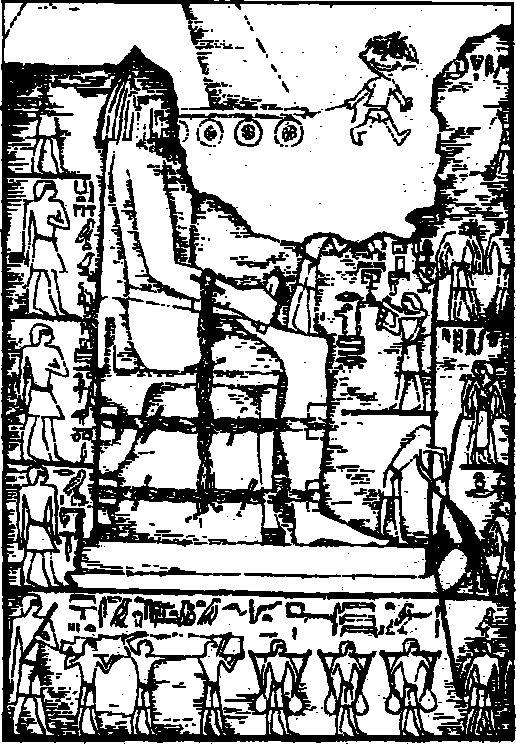
\includegraphics[width=\textwidth]{figures/fig-06-01.pdf}
\caption{Reducing the sliding friction by use of oil.}
\label{fig-6.1}
\end{figure}


\clearpage

The surface area does not occur in the above formula: the force of friction does not depend on the area of the contact surface between the bodies rubbing against each other. The same force is needed in order to set in motion, or to keep moving with a constant velocity, a wide sheet of steel weighing a kilogram and a kilogram weight which is supported by the surface of a small area.

And one more remark about forces of sliding friction. It is somewhat more difficult to set a body in motion than to keep it moving: the force of friction overcome at the first instant of motion, (static friction) exceeds the subsequent values by 20-30\%.

What can be said about the force of rolling friction, say, for a wheel? Just as for sliding friction, the greater the force that passes a wheel to a surface, the greater the rolling friction. Furthermore, the force of rolling friction is inversely proportional to the radius of the wheel. This is understandable: the larger the wheel, the less perceptible will be the roughness of the surface along which it is rolling.

If we compare the forces which must be overcome in making a body slide and roll, the difference we obtain is very impressive. For example, in order to pull a steel bar weighing 1 tonf along an asphalt pavement, a force of \SI{200}{\kgf} must be applied -- only an athlete is capable of doing this. But even a child can roll this very same bar on a cart -- a force not greater than \SI{10}{\kgf} is needed for this.

It’s no wonder that rolling friction has ``defeated'' sliding friction. It was not without reason that humanity switched to wheel transport a very long time ago.

The replacement of runners by wheels is not yet a com­plete victory over sliding friction, for a wheel must be attached to an axle. At first glance it seems impossible to avoid the friction of the axle on the bearings. So peo­ple thought during the course of centuries and tried to decrease the sliding friction in bearings only by means of various lubricants. The services rendered by lubricants have not been small -- sliding friction has been reduced by a factor of 8-10. But in a great many cases, the slid­ing friction, even with lubrication, is so considerable that it costs too much. This circumstance greatly impeded the development of technology at the end of the past century. It was then that the remarkable idea arose of replacing the sliding friction in bearings by rolling friction. Ball bearings have accomplished this replacement. Small balls were fitted in between the axle and the bush. As the wheel turns, the balls roll along the bush, and the axle rolls on the balls. The construction of this mechanism is shown in \figr{fig-6.2}. Sliding friction was replaced by rolling friction in this manner, thus reducing frictional forces tens of times over.

\begin{figure}[!ht]
\centering
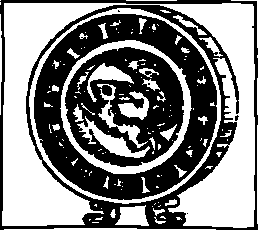
\includegraphics[width=0.4\textwidth]{figures/fig-06-02.pdf}
\caption{A ball bearing reduces sliding friction.}
\label{fig-6.2}
\end{figure}

The role played by ball and roller bearings in modern technology can scarcely be exaggerated. They are made with balls, with cylindrical rollers, with conical rollers. All machines, large and small, are equipped with such bearings. There exist ball bearings a millimetre in diam­eter; some bearings for large machines weigh over a ton. Balls for bearings (you have seen them, of course, in certain store windows) are manufactured with the most varying diameters -- from fractions of a millimetre to several centimetres.


\section{Viscous Friction in Liquids and Gases}

Until now we have been speaking of ``dry'' friction, i.e. of the friction arising from the contact of two solid objects. But floating and flying bodies are also subject to the action of frictional forces. The source of friction has changed -- dry friction is replaced by ``wet'' friction.

The resistance experienced by a body moving in water or air is subject to other laws, essentially different from the laws of dry friction, which we have spoken of above.

The rules for the behaviour of a liquid and a gas with respect to friction cannot be distinguished. Therefore, everything said below pertains to liquids and gases to the same degree. When we speak of a fluid, we will mean a liquid or a gas.

One of the distinctions between ``wet'' and dry friction consists in the absence of ``wet static friction'': an object suspended in water or air can, generally speaking, be started by an arbitrarily small force. But as for the fric­tional force experienced by a moving body, it will depend on the speed of the motion, on the form and dimensions of the body and on the properties of the fluid. The study of the motion of bodies in fluids has shown that there is no single law for ``wet'' friction, but there are two different laws: one is valid for motions with low speeds, and the other for motions with high speeds. The existence of two laws implies that the flow of a medium around a body moving in it takes place differently for motions of solids with high and low speeds.

For motions with low speeds, the force of resistance, or drag, is directly proportional to the speed and the linear dimensions of a body:
\begin{equation*}%
F \propto vL
\end{equation*}
How should we understand the proportionality to dimension if we aren’t told what shape the body has?

What is meant is that for two bodies completely similar in shape (i.e. all of whose corresponding dimensions are in the same ratio), the ratio of the drag is the same as that of the linear dimensions of the bodies.

Drag depends to an enormous degree on the properties of a fluid. Comparing the frictional forces experienced by the same objects moving with identical speeds in various media, we see that the thicker or, as we say, the more viscous the medium, the greater the drag experienced by a body. It is therefore appropriate to call the friction under discussion \emph{viscous friction}. It is quite understandable that air creates a negligible viscous friction, approx­imately 60 times less than water. A liquid can be ``thin'', like water, or very viscous, like sour cream and honey.

We can judge the degree of viscosity of a liquid either by the speed with which solid bodies fall in it or by the speed with which it pours through an opening.

It will take water several seconds to pour out of a half­ litre funnel. A very viscous liquid will trickle out of it in hours, or even days. It is possible to give examples of even more viscous liquids. Geologists have called atten­tion to the fact that in the craters of certain volcanoes spherical pieces are found in accumulations of lava on the inner sides. At first sight, it was completely impossible to understand how such a sphere might be formed out of lava inside a crater. This would be incomprehensible if lava were regarded as a solid. But if lava behaves like a liquid, it will drop down the crater just like any other liquid. But only a drop will be formed not in a fraction of a second but in the course~of decades. When the drop becomes too heavy, it will break away and fall at the bottom of the crater.

It is clear from this example that real solid bodies and amorphous bodies, which, as we know, resemble liquids much more than crystals, should not be put on the same level. Lava is precisely such an amorphous body. It seems
to be solid, but is actually a very viscous liquid.

What do you think, is sealing wax a solid? Take two corks and place them at the bottom of two cups. Pour any melted salt (for example, saltpeter -- it is easily obtained) into one, and pour sealing wax into the other cup with a cork. Both liquids will harden and bury the corks. Put these cups away in the cupboard and forget about them for a long time. After several months, you will see the difference between sealing wax and salt. The cork drowned in salt will be at rest, as before, at the bottom of its cup. But the cork drowned in sealing wax will turn out to be on the top. But how did this occur? Very simply: the cork came to the surface in quite the same way as it would do in water. The only difference being is that of time: when the force of viscous friction is small, a cork comes to the surface instantly, but in very viscous liquids floating up takes months.

\section{Forces of Resistance at High Speeds}

But let us return to the laws of ``wet'' friction. As we explained, at low speeds the drag depends on the viscosity of a liquid, the speed of the motion and the linear dimen­sions of a body. Let us now consider the laws of friction for high speeds. But first of all, we must say what speeds are to be regarded as low, and what speeds as high. We are interested not in the numerical value of the speed but in whether the speed is sufficiently low for the law of viscous friction considered above to hold.

It turns out that it is impossible to name a number of metres per second such that the laws of viscous friction be applicable in all cases with lower speeds. The bounds of applicability of the law we have studied depends on the dimensions of a body and on the degree of viscosity and density of a liquid.

For air, ``low'' is a speed less than
\begin{equation*}%
\frac{0.75}{L}\, \si{\centi\meter\per\second}
\end{equation*}
for water, less than
\begin{equation*}%
\frac{0.05}{L} \, \si{\centi\meter\per\second}
\end{equation*}
and for viscous liquids like thick honey, less than
\begin{equation*}%
\frac{100}{L} \, \si{\centi\meter\per\second}
\end{equation*}
Consequently, the laws of viscous friction are scarcely applicable to air and especially to water: even for low speeds, of the order of \SI{1}{\centi\meter\per\second}, they will apply only for tiny bodies with millimetre dimensions. The resistance experienced by a person diving into water is to no extent subject to the law of viscous friction.

But how can we explain the fact that the law governing the resistance of a medium changes with a change in speed? The causes must be sought in the change in the character of the flow of a liquid around a body moving in it. Two circular cylinders moving in a liquid are de­picted in \figr{fig-6.3} (their axes are perpendicular to the drawing). For a slow motion, the liquid flows smoothly around the moving object -- the drag which it has to overcome is the force of viscous friction (\figr{fig-6.3}~\hlgray{a}). For a high speed, behind the moving body there arises a complicated irregular motion of the liquid (\figr{fig-6.3}~\hlgray{b}). Var­ious streams appear and disappear, forming fantastic figures, rings and eddies. The picture made by the streams is changing all the time. The appearance of this motion, called turbulent, radically changes the law of resistance.
\begin{figure}[!ht]
\centering
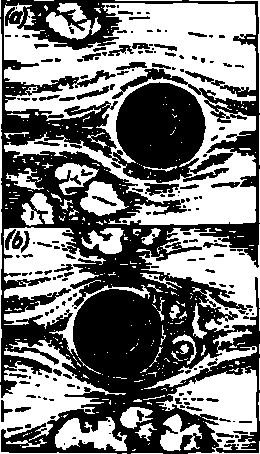
\includegraphics[width=0.6\textwidth]{figures/fig-06-03.pdf}
\caption{Laminar and turbulent flows.}
\label{fig-6.3}
\end{figure}

Turbulent resistance depends on the speed and dimen­sions of an object in an entirely different way than vis­cous resistance: it is proportional to the square of the speed and the square of the linear dimensions. The vis­cosity of a liquid during this motion ceases to play an essential role; the determining property becomes its density, with the drag proportional to the first power of the density of the fluid. Therefore, the following formula holds for the force $F$ of turbulent resistance:
\begin{equation*}%
F \propto \rho v^{2} L^{2}
\end{equation*}
where $v$ is the speed of the motion, $L$ are linear dimensions of the object, and $\rho$ is the density of the medium. The numerical proportionality factor, which we haven’t written down, has various values depending on the shape of the body.


\section{Streamline Shape}

Motion in the air, as has been said above, is almost always ``speedy'', i.e. the basic role is played by turbulent and not viscous resistance. Airplanes, birds and parachut­ists experience turbulent resistance. If a person falls through the air without a parachute, then after a certain time he begins falling uniformly (the force of resistance balances the weight), but with quite a considerable speed, of the order of \SI{50}{\meter\per\second}. The opening of a parachute leads to a sharp deceleration of the fall -- the same weight is now balanced by the resistance of the canopy. Since the force of resistance is proportional to the speed of the mo­tion as well as to the linear dimensions of the falling object, the speed will decrease as many times as the linear dimensions of the falling body increase. The diameter of a parachute is about \SI{7}{\meter}, whereas the ``diameter'' of a man’s body is about one metre. The speed of the fall will be decreased to \SI{7}{\meter\per\second}. One can land safely with such a speed.

We must say that the problem of increasing the re­sistance is far more easily solved than the converse prob­lem. Reducing the air resistance on a car or an airplane, or the water resistance on a submarine, is one of the most important and difficult technological problems.

It proves possible to decrease turbulent resistance by a large factor by changing the shape of a body. For this one must reduce to a minimum the turbulent motion, which is the source of the resistance. This is achieved by, as they say, streamlining the object.

But what shape is best in this sense? It would appear at first sight that the body should be shaped so that the forward side comes to a point. Such a point, it seems, should ``cleave'' the air most successfully. But it proves important not to cleave the air but to disturb it as little as possible so that it flows smoothly around the object.

The best profile for a body moving in a fluid is the one whose shape is obtuse in front and pointed behind.\footnote{The pointed prows of boats and sea-going vessels are needed for ``breaking'' waves, i.e. only when the motion is taking place along the surface.} With such a shape, the fluid would flow smoothly off the point and turbulence would be reduced to a minimum. Sharp edges should not in any case be put in front, since there they would create turbulence.
\begin{figure}[!ht]
\centering
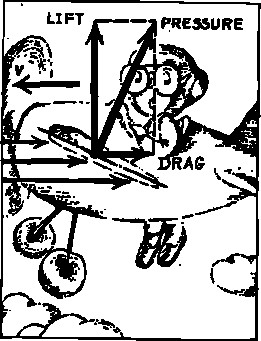
\includegraphics[width=0.4\textwidth]{figures/fig-06-04.pdf}
\caption{Lift, pressure and drag for a flying body.}
\label{fig-6.4}
\end{figure}

The streamline shape of an airplane wing creates not only the least resistance to the motion but also the great­est lift, when the fairing is inclined upwards from the direction of the motion. Flowing around a wing, the air pushes against it mainly in the direction perpendicular to its plane (\figr{fig-6.4}). It is clear that for an inclined wing this force is directed upwards.

The lift grows with an increase in the angle of attack. But reasoning based solely on geometrical considerations would lead us to the false conclusion that the greater the angle of attack, the better. But as a matter of fact, as the angle of attack is increased, the smooth flow of the plane becomes more and more difficult, and at a certain value for this angle, as illustrated in \figr{fig-6.5}, violent turbulence arises; the drag sharply increases and the lift decreases.

\begin{figure}[!ht]
\centering
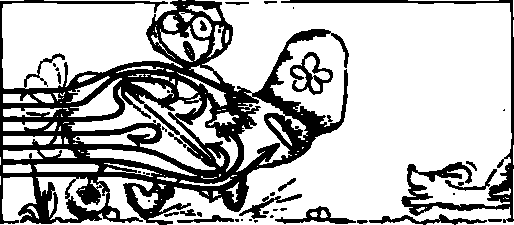
\includegraphics[width=\textwidth]{figures/fig-06-05.pdf}
\caption{Angle of attack and flight of plane.}
\label{fig-6.5}
\end{figure}

\section{Disappearance of Viscosity}

Very often, in explaining some phenomenon or describ­ing the behaviour of one or another group of bodies, we refer to well-known examples. It is quite obvious that this object should be moving in such a manner, we say, for other bodies also move according to the very same rules. The explanation reducing the new to that which we have already come across in the course of our lives always satisfies the majority. We therefore did not have any particular difficulty in explaining to the reader the laws in accordance with which liquids move -- for everyone has seen how water flows, and the laws governing this motion seem quite natural.

However, there is one perfectly amazing liquid which does not resemble any other liquid and moves in accor­dance with special laws characteristic of it alone. It is liquid helium.

We have already said that liquid helium remains in the liquid phase right down to the temperature of absolute zero. However, helium above \SI{2}{\kelvin} (more precisely, \SI{2.19}{\kelvin}) and helium below this temperature are two completely different liquids. Above two degrees, the properties of helium in no way distinguish it from other liquids. Below this temperature, helium becomes a miraculous liquid. This miraculous helium is called helium II.

The most striking property of helium II is its \emph{super­ fluidity}, i.e. complete lack of viscosity, discovered by P. L. Kapitza in 1938.

In order to observe superfluidity, a vessel is made with a very fine slit at the bottom -- of only half a micrometre in width. An ordinary liquid hardly seeps through such a slit; helium also behaves this way at temperatures above \SI{2.19}{\kelvin}. But as soon as the temperature becomes barely less than \SI{2.19}{\kelvin}, the speed with which helium flows out of such a vessel grows by leaps and bounds -- by a factor of at least several thousand. Helium II almost momentarily flows through the narrowest clearance, i.e. it com­pletely loses its viscosity. The superfluidity of Helium leads to an even stranger phenomenon. Helium II is ca­pable of ``climbing out'' of the glass or test tube into which it was poured. A test tube with helium II is placed in a Dewar vessel over a helium bath. ``Without rhyme or reason'', helium rises along the wall of the test tube in the form of a very fine, completely unnoticeable film and overflows; drops fall from the bottom of the test tube.

It should be recalled that thanks to capillary forces, which were discussed on page~\pageref{capillary-force}, the molecules of every liquid wetting the wall of a vessel climb up this wall and form the finest film on it whose width is of the order of \SI{d-6}{\centi\meter}. This film cannot be seen by an eye, and in gener­al does not manifest itself in any way for an ordinary viscous liquid.

The picture changes completely if we are dealing with helium devoid of viscosity. In fact, a narrow slit does not hinder the movement of superfluid helium, and a thin film on a surface is just the same as a narrow slit. A liquid without viscosity flows in a very fine layer. The film cov­ering the surface forms a siphon over the edge of the glass or test tube through which the helium overflows the vessel.

It is obvious that we do not observe anything of the kind in the behaviour of an ordinary liquid. A liquid of standard viscosity is practically unable to ``make its way'' through a siphon of negligible thickness. Such a motion is so slow that the outflow would last millions of years.

Thus, helium II is devoid of any viscosity. The conclu­sion that a solid should move without friction in such a liquid would appear to follow from this with iron logic. Let us take a disc on a string, place it in liquid helium II and twist the string. Leaving this uncomplicated device alone, we create something like a pendulum -- the string with the disc will oscillate and periodically twist first in one and then in another direction. If there were no friction, we should expect the disc to oscillate perpet­ually. But nothing of the kind! 

After a comparatively short time, approximately the same as for ordinary helium I (i.e. helium at a temperature above \SI{2.19}{\kelvin}), the disc comes to a halt. But how will this happen? When flowing through a slit, helium behaves like a liquid without vis­cosity, but behaves like an ordinary viscous liquid in relation to bodies moving in it. It is this, to be sure, that is in fact completely extraordinary and incomprehensible. It now remains for us to recall that helium does not solidify right up to absolute zero. The crux of the problem is that the ideas about motion which we are accustomed to are not suitable any more. If helium has remained liquid ``illegally'', should we be surprised by the lawless behaviour of this liquid?

It is only possible to understand the behaviour of liquid helium from the point of view of the new concep­tions of motion, quantum mechanics. Let us try to give a general idea of how quantum mechanics explains the behaviour of liquid helium.

Quantum mechanics is an extremely intricate theory, which is very hard to understand, and so the reader should not be surprised that the explanation looks even stranger than the phenomena themselves. It turns out that every particle of liquid helium participates simultaneously in two motions: one motion is superfluid, unrelated to vis­cosity, and the other is ordinary.

Helium II behaves as if it consisted of a mixture of two liquids moving completely independently, ``one through the other''. One liquid behaves normally, i.e. possesses an ordinary viscosity, while the other component part is superfluid.

When helium flows through a slit or overflows a glass, we observe the effect of superfluidity. But during the oscillation of a disc submerged in helium, friction is created because it is inevitable in the normal part of helium.

The ability to participate in two distinct motions also gives rise to completely unusual heat-conducting proper­ ties of helium. As has been already said, liquids in general conduct heat rather poorly. Helium I also behaves like an ordinary liquid. But when the transformation into he­lium II takes place, its thermal conductivity grows about a thousand million-fold. Therefore, helium II conducts heat better than the best ordinary heat conductors, such as copper and silver.

The fact is that the superfluid motion of helium does not participate in the heat transfer. Consequently, when there is a difference in temperature within helium II, there arise two currents in opposite directions, and one of them -- the normal one -- carries heat with it. This does not at all resemble ordinary thermal conductivity. In an ordinary liquid, heat is transferred by means of mo­lecular collisions. In helium II, heat flows together with the ordinary part of helium -- flows like a liquid. Here at last the term ``heat flow'' is fully justified. It is pre­cisely such a method of transferring heat that leads to an immense thermal conductivity.

This explanation of the thermal conductivity of helium may seem so strange that you will refuse to believe it. But it is possible to convince oneself first-hand of the validity of what has been said by means of the following conceptually simple experiment.

In a tub with liquid helium there is a Dewar vessel filled to the brim with helium. The vessel is connected to the tub by means of a capillary branch piece. The helium in­ side the vessel is heated by an electric spiral, but heat does not pass to the surrounding helium through the walls of the vessel, since they do not transmit heat. Near the end of the capillary tube there is a vane suspended on a fine thread. If the heat is flowing like a liquid, it should turn the vane. This is precisely what happens. Moreover, the amount of helium in the vessel does not change. How can this miraculous phenomenon be explained? In only one way: during heating there arises a current of the nor­mal part of the liquid from the heated place to the cold, and a current of the superfluid part in the opposite di­rection. The amount of helium at each point does not change, but since the normal part of the liquid moves together with the heat transfer, the vane turns as a re­sult of the viscous friction of this part and remains de­flected as long as heating continues.

Another conclusion also follows from the fact that su­perfluid motion does not transfer heat. We have spoken above about the ``creeping'' of helium over the brim of a glass. But the superfluid part ``climbs out'' of the glass, while the normal part remains there. Heat is connected to only the normal part of helium and does not accompany the superfluid part which is climbing out of the glass. Hence, as helium climbs out of the vessel, one and the same amount of heat will be shared by a smaller and smaller amount of helium -- the helium remaining in the vessel should warm up. This is actually observed during experiments.

The masses of the helium partaking in superfluid and normal motion are not identical. Their ratio depends on the temperature. The lower the temperature, the greater the superfluid part. All of the helium becomes superfluid at absolute zero. As the temperature rises, a larger and larger part of the helium begins to behave normally, and at the temperature of 2.19 K, all of the helium becomes normal, acquiring the properties of an ordinary liquid.

But the reader already has some questions in his mind: What precisely is called superfluid helium, how can a particle of liquid participate simultaneously in two mo­tions and how can the very fact of two motions of a single particle be explained?\ldots{} Unfortunately, we are obliged to leave all these questions unanswered. The theory of helium II is too complicated, and it is necessary to know a great deal in order to understand it.

\section{Plasticity}

\emph{Elasticity} is the ability of a body to recover its form after a force ceased acting on it. If a kilogram weight is hung on a \SI{1}{\meter} steel wire with a cross-sectional area of \SI{1}{\milli\meter\squared}, the wire will be stretched. The stretching is ne­gligible, only  \SI{0.5}{\milli\meter} in all, but it is not difficult to observe. If the load is removed, the wire will contract by the same \SI{0.5}{\milli\meter}, and so its length will return to its former value. Such a deformation is called \emph{elastic}.

Let us note that a wire of \SI{1}{\milli\meter\squared} cross-section under the action of a force of \SI{1}{\kgf} and a wire of \SI{1}{\centi\meter\squared} cross-section under the action of a force of \SI{100}{\kgf} are, as one says, under the same conditions of mechanical stress. Therefore, the behaviour of a material must always be described by indicating not the force (which would be pointless if the cross-section of a body is unknown), but the stress, i.e. the force per unit of area. Ordinary bodies -- metals, glass, stones -- can be stretched elastically by only several per cent at best. Rubber possesses outstanding elastic properties. Rubber can be stretched elastically by several hundred per cent (i.e. made two or three times longer than it was originally), and when we let such a rubber band go, we see that it returns to its initial state.

All bodies without exception behave elastically under the action of small forces. However, a limit of elasticity appears earlier for some bodies and considerably later for others. For example, the elastic limit for such soft metals as lead has already been reached when a load of 0.2-0.3 \si{\kgf} is hung on a wire of \SI{1}{\milli\meter\squared} cross-section. This limit is approximately 100 times as great, i.e. about \SI{25}{\kgf}, for such hard materials as steel.

With respect to large forces exceeding the elastic limit the various bodies can be roughly divided into two classes: those like glass, i.e. fragile, and those like clay, i.e. plastic.

If you press a piece of clay with your finger, it will leave its imprint, containing even the intricate whirls drawn on its skin. If you strike a piece of soft iron or lead with a hammer, a clear trace will be left. There is no longer any force, but the deformation remains -- it is called \emph{plastic} or \emph{permanent}. You will not succeed in ob­taining such residual effects with glass: if you persist in this endeavour, the glass will break. Certain metals and alloys, such as cast iron, are just as fragile. An iron pail will flatten, but a cast iron pot will crack, under the blows of a hammer. One can judge the strength of fragile bodies by the following figures. In order to convert a piece of cast iron into powder, one must act with a force of about 50-80 \si{\kgf} per square millimetre of surface area. This figure falls to 1.5-3 \si{\kgf} for a brick.

As for every classification, the division of bodies into fragile and plastic is, to a fair degree, relative. First of all, a body which is fragile at a low temperature can be­ come plastic at higher temperatures. Glass can be superb­ly processed as a plastic material if it is heated to a temperature of several hundred degrees. Soft metals, such as lead, can be forged cold, but hard metals yield to forging only when burning hot. A rise in temperature sharply increases the plasticity of a material.

One of the essential features of metals, which has made them irreplaceable building materials, is their hardness at room temperatures and plasticity at high temperatures: an incandescent metal can be easily given the required form, but it is only possible to change this form at room temperature by means of very substantial forces.

The internal structure of a material influences its me­chanical properties in an essential way. It is obvious that cracks and holes weaken the apparent strength of a body and make it more fragile.

The ability of plastically deformable bodies to strengthen is remarkable. A single crystal of a metal is very soft when it has just grown up out of a melt. Crystals of many metals are so soft that they are easily bent with one’s fingers; however, one will not succeed in straightening them out. Strengthening has taken place. This same spec­imen can now be plastically deformed only by means of a considerably greater force. It turns out that plasticity is not only a property of a material, but also a prop­erty of its treatment.

Why are instruments made not by casting metals, but by forging them? The reason is obvious -- a metal subjected to forging (or rolling, or drawing) is much stronger than cast metal. No matter how much we forge a metal, we cannot increase its strength beyond a certain limit, which is called the yield stress. For steel it is between 30 and \SI{50}{\kgf\per\milli\meter\squared}. This figure has the following meaning. If a one-pood weight (below the yield stress) is hung on a wire of \SI{1}{\milli\meter\squared} cross-section, the wire will begin stretching and strengthening simultaneously. The stretching will therefore quickly cease -- the weight will hang calmly on the wire. But if a two- or three-pood weight (above the yield stress) is hung on such a wire, the picture will be different. The wire will keep stretching until it breaks. Let us emphasize once again that the mechanical behav­iour of a body is determined not by the force, but by the stress. A wire of a cross-section of \SI{100}{\micro\meter\squared}will yield under the action of a load of (30-50) $\times \SI{d-4}{\kgf}$, i.e. 3-5~gf.

\section{Dislocations}

Proving that plastic deformation is a phenomenon of immense significance in engineering practice would be forcing an open door. Smith and die forging, rolling sheets, drawing wire are all techniques based on the plastic work­ ing of metals leading to their deformation.

We could understand nothing about plastic deforma­tion if we considered the crystallites of which a metal con­sists to be ideal fragments of space lattices.

The theory of the mechanical properties of an ideal crystal was worked out long ago, at the beginning of the century. This theory disagrees with experimental data about a thousand-fold. If all crystals were ideal, their tensile strength would be many orders of magnitude high­er than that actually observed. Then plastic deformation would require huge forces.


Hypotheses had been suggested much earlier than sufficient facts accumulated to support them. It was obvious to investigators that the only way to reconcile theory with practice was to assume that crystallites have certain defects. Various conjectures could be made, of course, on the nature of these defects. But the picture began to clear up only after the most sophisticated equipment for investigating the structure of matter had been made available to physicists. It was found that an ideal portion of a lattice (called a block) has dimensions of the order of several millionths of a centimetre. These blocks are disoriented with respect to one another by angles within a second or a minute of arc.
\begin{figure}[!ht]
\centering
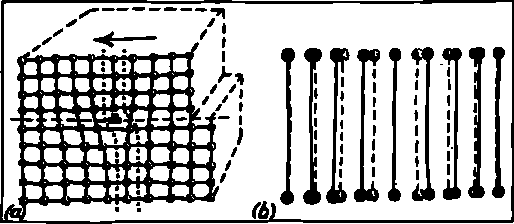
\includegraphics[width=\textwidth]{figures/fig-06-06.pdf}
\caption{A simple or linear dislocation in crystals.}
\label{fig-6.6}
\end{figure}

Many facts accumulated by the end of the twenties led to the important contention that the chief (though not only) defect of a real crystal is a regular displacement that was named a \emph{dislocation}. A simple, or linear, dislocation is illustrated by the model in \figr{fig-6.6}. The essence of the defect, as is evident, is that there are places in the crystal that seem to contain an ``extra'' atomic plane (from which its name ``extraplane'' is derived). The horizontal dash line in \figr{fig-6.6}~\hlgray{(a)} divides two blocks. The upper part of the crystal is in compression, and the lower part in tension. The effect of the dislocation on the crystal is rapidly dissipated as seen in \figr{fig-6.6}~\hlgray{(b)} which is a sort of ``top'' view of the left-hand drawing. 

Another type of dislocation, frequently found in crystals, is the screw dislocation. It is illustrated schemati­cally in \figr{fig-6.7}. Here the lattice is divided into two blocks, one of which has slipped, as it seems, by one lattice constant with respect to the other. Maximum distortion is concentrated at the vertical axis shown in the diagrams. The region adjoining this axis is what is called a screw dislocation.
\begin{figure}[!ht]
\centering
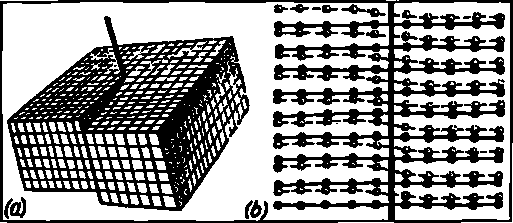
\includegraphics[width=\textwidth]{figures/fig-06-07.pdf}
\caption{The screw dislocation in crystals.}
\label{fig-6.7}
\end{figure}

We shall understand the nature of this distortion better if we look at the other diagram ( \figr{fig-6.7}~\hlgray{(b)}), which illus­trates two adjacent atomic planes on the two sides of the vertical plane passing through the axis (the one along which slip has occurred). With respect to the three-dimensional view, this is a projection showing the plane from the right. Here we see the axis of the screw disloca­tion, the same as in the other drawing. The atomic plane belonging to the right-hand block is shown by full lines; that belonging to the left-hand block by dash lines. The black circles are closer to the reader than the light ones. It is evident from the drawing that a screw dislocation is another type of distortion differing from that of a linear distortion. There is no extra row of atoms. The essence of the distortion is that the rows of atoms change their nearest neighbours near the dislocation axis. They are bent downwards to align themselves with the neighbours located one storey below.

Why is this called a screw dislocation? Imagine that you are strolling along the atoms (after reducing your size to subatomic dimensions) and have decided to pass around the dislocation axis. It is obvious that if you start your journey on the lowest plane you will find your­ self one storey higher after each turn. Finally, you will emerge on the top surface of the crystal, as if you had been climbing winding stairs in a helix like the thread of a screw. In our drawing, the climb is in the counter­ clockwise direction. If the slip of the blocks had been in the opposite direction, your journey would have been clockwise.

We are now ready to answer the question of how plastic deformation takes place.

Assume that we want to shift the upper half of a crystal with respect to the lower one by one interatomic distance. Evidently, we must roll all the atoms in the shear plane over one another. It is an entirely different matter when a shear force acts on a crystal containing a dislocation.

\begin{figure}[!ht]
\centering
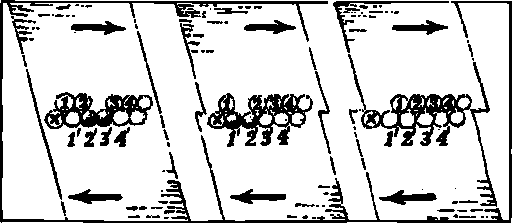
\includegraphics[width=\textwidth]{figures/fig-06-08.pdf}
\caption{Close packing arrangement of spheres.}
\label{fig-6.8}
\end{figure}


\figr{fig-6.8} illustrates a close packing arrangement of spheres (only the end spheres of the rows of atoms are shown), containing a linear dislocation, consisting of a linear void (something like a fissure) between two of the upper rows. We begin to shift the upper block to the right with respect to the lower one. To help you understand what is happening, we have given numbers to the rows, with primed numbers for the spheres of the com­ pressed (lower) layer. At some initial moment, the ``fissure'' is between rows \textbf{2} and \textbf{3}; the compressed rows are \textbf{2'} and \textbf{3'}. As soon as the shifting force is exerted, row \textbf{2} moves into the ``fissure''; now row \textbf{3'} can ``breathe freely'', but row \textbf{1'} will have to squeeze into less space. What happened? The whole dislocation moved to the left, and its mo­tion continues in the same way until it (the dislocation) ``emerges'' from the crystal. The result is a shift over one row of atoms, i.e. the same as in the shear of a perfect crystal.

It is evidently unnecessary to prove that shear by dislocation motion requires much less force. In the shear of a perfect crystal we had to overcome the interaction be­ tween atoms in rolling over all the rows simultaneously. In dislocation shear, only a single row of atoms is involved at each instant.

Calculations indicate that the strength of crystals in shear, assuming there are no dislocations, should be a hundred times more than that actually observed in ex­periments. The presence of even a slight number of dis­ locations can reduce the strength of the material by a substantial factor.
The preceding discussion poses a question that must be cleared up. It is evident from the drawing (see \figr{fig-6.8}) that the applied force ``drives'' the dislocation out of the crystal. This implies that the crystal becomes stronger and stronger as we increase the degree of deformation. Finally, when the last dislocation is eliminated, the crys­tal should, according to the theory, become about a hundred times stronger than a perfect regular crystal. The crystal actually is strengthened in the course of deformation, but far from a hundred-fold. The screw dis­ locations save the day. It was established (and here the reader will just have to take our word for it because it is so difficult to illustrate with a drawing) that screw dis­ locations cannot be easily ``driven'' out of a crystal. More­over, shear of the crystal may take place with the aid of dislocations of both types. Dislocation theory satis­ factorily explains the features of shear phenomena along crystal planes. According to up-to-date views, plastic deformation of crystals consists in the motion of disorder
along the crystal.

\section{Hardness}

Strength and hardness do not go hand in hand with each other. A rope, a scrap of cloth and a silk thread can possess a great deal of strength -- a considerable stress is needed to tear them. Of course, nobody will say that rope and cloth are hard materials. And conversely, the strength of glass is not great, but glass is a hard material.

The concept of hardness used in technology is taken from everyday practice. \emph{Hardness} is the resistance to pen­etration. A body is hard if it is difficult to scratch it, difficult to leave an imprint on it. These definitions may seem somewhat vague to the reader. We are accustomed to physical concepts being expressed in terms of numbers. But how can this be done in relation to hardness?

One rather primitive method, which is nevertheless use­ful in practice, has already been employed for a long time by mineralogists. Ten definite minerals are arranged in a series. The first is diamond, followed by corundum, then topaz, quartz, feldspar, apatite, fluor-spar, calcite, gyp­sum and talc. The series is sorted out in the following manner: diamond leaves its mark on all minerals, but none of these minerals can scratch diamond. This means that diamond is the hardest mineral. The hardness of diamond is evaluated by the number 10. Corundum, which follows diamond in the series, is harder than all the min­erals below it -- corundum can scratch them. Corundum is assigned the hardness number 9. The numbers 8,7 and 6 are assigned to topaz, quartz and feldspar, respectively, on the same grounds. Each of them is harder than (i.e. can scratch) all the minerals below it, and softer than (can itself be scratched by) the minerals having greater hardness numbers. The softest mineral, talc, has hardness number 1.

A ``measurement'' (this word must be taken in quotation marks) of hardness with the aid of this scale consists in finding the place for the mineral of interest to us in a series containing the ten chosen standards. If the unknown mineral can be scratched by quartz, but leaves its mark on feldspar, its hardness is equal to 6.5.

Metallurgists use a different method for determining hardness. A dent is made on the material being tested by pressing a steel ball \SI{1}{\centi\meter} in diameter against it with a standard force (ordinarily \SI{3000}{\kgf}). The radius of the small pit so formed is taken as the hardness number.

Hardness with respect to scratching and hardness with respect to pressing do not necessarily correspond, and one material may prove to be harder than another when tested by scratching but softer when tested by pressing.

Consequently, there is no universal concept of hardness independent of the method of measurement. The concept of hardness is a technological and not a physical con­cept.

\section{Sound Vibrations and Waves}

We have already given the reader a lot of information about oscillations. How a pendulum and a ball on a spring oscillate and what regularities there are in the oscillation of a string, all of this was studied in one of the chapters of the first book. We haven’t spoken about what takes place within the air or some other medium when a body located in it performs oscillations. There is no doubt that the medium cannot remain indifferent to vibrations. An oscillating object pushes the air, displacing the air particles from the positions in which they were previously located. It is also obvious that this cannot be limited to the influence on only the adjacent layer of air. The body will push the nearest layer, this layer presses against the next one, and so layer after layer, particle after particle, all of the surrounding air is brought into motion. We say that the air has come to a vibrating state, or that \emph{sound vibrations} are taking place in the air.

We call the vibrations of the medium sound vibrations, but this does not mean that we hear all of them. Physics uses the concept of sound vibrations in a broader sense. The question as to which sound vibrations are heard will be discussed below.

We are dealing with air only because sound is most of­ ten transmitted through air. But there are, of course, no special properties of air which would give it a monopoly to perform sound vibrations. Sound vibrations arise in any medium capable of being compressed, but since there are no incompressible bodies in nature, the particles of any material can therefore find themselves in this state. The study of such vibrations is usually called \emph{acoustics}.

Each particle of air remains at one place, on the av­erage, during sound vibrations -- it only performs oscilla­tions about its equilibrium position. In the simplest case, a particle of air can perform a harmonic oscillation, which, as we recall, takes place in accordance with the sinusoidal law. Such an oscillation is characterized by the maximum displacement of a particle from its equilibrium position (amplitude) and the period of the oscillation, i.e. the time required to perform a complete oscillation.

The concept of the \emph{frequency of vibration} is used more often than that of the period for describing the properties of sound vibrations. The frequency $\nu = 1/T$ is the recip­rocal of the period. The unit of frequency is the inverse second (\si{\per\second}). If the frequency of vibration is equal to \SI{100}{\per\second}, this means that during one second a particle of air performs 100 complete vibrations. Since in physics we must deal rather often with frequencies which are many times greater than a hertz, the units \emph{kilohertz} and \emph{megahertz} are widely applied; $\SI{1}{\kilo\hertz} = \SI{d3}{\kilo\hertz},\,\, \SI{1}{\mega\hertz} = \SI{d6}{\hertz}$.

The speed of a vibrating particle is maximum when it is passing through its equilibrium position. On the con­trary, in positions of maximum displacement, the speed of a particle is, naturally, equal to zero. We have already said that if the displacement of a particle is subject to the law of harmonic oscillation, the change in its speed of vibration obeys the same law. If we denote the maximum value (amplitude) of the displacement by $s_{0}$, and of the speed by $v_{0}$ then $v_{0}= 2 \pi s_{0}/T$, or $v_{0}= 2 \pi \nu s_{0}$. Loud con­versation brings air particles into vibration with an amplitude of only several millionths of a centimetre. The maximum value of the speed will be of the order of \SI{0.02}{\centi\meter\per\second}.

Another important physical quantity varying together with the displacement and speed of a particle is the \emph{excess pressure}, also called the \emph{sound pressure}. A sound vibration of air consists in a periodic alternation of compression and rarefaction at each point in the medium. The air pressure at any place is now higher, now lower than the pressure which would be there in the absence of sound. This excess (or insufficiency) of pressure is just what is called the sound pressure. Sound pressure is a small fraction of standard atmospheric pressure. For a loud conversation the sound pressure amplitude will be equal to approxi­mately one-millionth of the atmospheric pressure. Sound pressure is directly proportional to the speed of the vibra­tion of a particle, where the ratio of these physical quantities depends only on the properties of the medium. For example, a speed of vibration of \SI{0.025}{\centi\meter\per\second} corresponds to a sound pressure in air of \SI{1}{\dyne\per\centi\meter\squared}.

\begin{figure}[!ht]
\centering
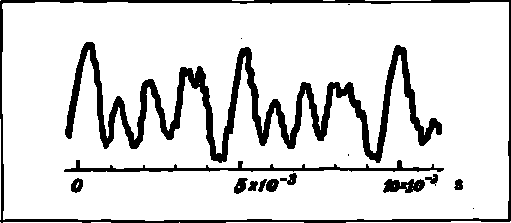
\includegraphics[width=\textwidth]{figures/fig-06-09.pdf}
\caption{A graph of sound vibrations.}
\label{fig-6.9}
\end{figure}

A string vibrating in accordance with a sinusoidal law brings air particles into harmonic oscillation. Noises and musical sounds lead to a considerably more complicated picture. A graph of sound vibrations, namely of the sound pressure as a function of time, is shown in \figr{fig-6.9}. This curve bears little resemblance to a sine wave. It turns out, however, that any arbitrarily complicated vibration can be represented as the result of superposing a large number of sine waves with different amplitudes and frequencies. These simple vibrations make up, as is said, the spectrum of the complex vibration. Such a su­perposition of vibrations is shown for a simple example in \figr{fig-6.10}.
\begin{figure}[!ht]
\centering
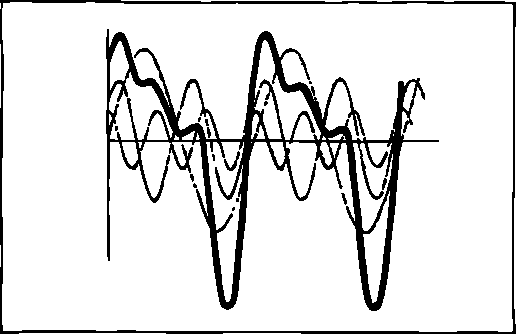
\includegraphics[width=\textwidth]{figures/fig-06-10.pdf}
\caption{A graph of superposition of sound waves.}
\label{fig-6.10}
\end{figure}

If sound were propagated instantaneously, all the air particles would vibrate in unison. But sound is not prop­agated instantaneously, and the masses of air lying on the lines of propagation are brought into motion in turn, as if caught up by a wave coming from some source. In exactly the same way, a chip lies calmly on the water until the circular waves from a pebble thrown into the water catch it up and make it vibrate.

Let us confine our attention to a single vibrating par­ticle and compare its behaviour with the motion of other particles lying on the same line of sound propagation. An adjacent particle will start vibrating somewhat later, the next particle still later. The delay will keep increasing until we meet a particle which is lagging behind by a whole period and is therefore vibrating in time with the initial particle. So an unsuccessful runner, who has fallen behind the leader by an entire lap, can cross the finish line simultaneously with the leader. But at what distance will we meet the point which is vibrating in time with the initial particle? It is not hard to see that this distance $\lambda$ is equal to the product of the speed of propagation of sound $c$ by the period of vibration $T$. The distance $\lambda$ is called the \emph{wavelength}:
\begin{equation*}%
\lambda = c T
\end{equation*}
We will find points vibrating in time after intervals of length $\lambda$. Points separated by a distance of $\lambda/2$ will move relative to each other like an object vibrating perpendic­ularly to a mirror moves with respect to its image.

If we depict the displacement (or speed, or sound pres­sure) of all the points lying on a line of propagation of a harmonic sound, then a sine wave is again obtained.

\begin{figure}[!ht]
\centering

\includegraphics[width=0.5\textwidth]{figures/fig-06-11.pdf}
\caption{A graph of amplitude vs. time for sound waves.}
\label{fig-6.11}
\end{figure}

The graphs of the wave motion and the vibration should not be confused. There is a strong resemblance between \figr{fig-6.11} and \figr{fig-6.12}, but the distance is plotted along the horizontal axis in the former, while the time in the latter. One figure represents the development of the vibration in time, and the other an instantaneous ``photograph'' of the wave. It is evident from the comparison of these two graphs that the wavelength may also be called its spatial period: the quantity $\lambda$ plays the same role in space as $T$ plays in time.

\begin{figure}[!ht]
\centering
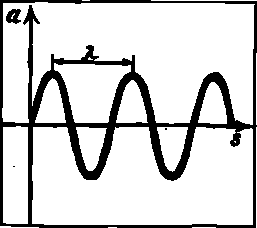
\includegraphics[width=0.5\textwidth]{figures/fig-06-12.pdf}
\caption{A graph of amplitude vs. distance for sound waves.}
\label{fig-6.12}
\end{figure}

In a graph of a sound wave, the displacements of a particle are plotted along the vertical axis, and the hor­izontal axis is the direction of the propagation of the wave along which the distance is marked off. This might suggest the false idea that the particles are displaced per­pendicularly to the direction of the propagation of the wave. In reality, air particles always vibrate along the direction of the propagation of the sound. Such a wave is called \emph{longitudinal}.

The speed of light is incomparably greater than that of sound; light is propagated practically instantaneously. Thunder and lightning occur at the same instant; we see a flash of lightning practically at the instant of discharge, but the sound of thunder reaches us at a speed of approx­imately one kilometre in three seconds (the speed of sound in air is \SI{330}{\meter\per\second}). Hence, when we hear the thunder, there is no longer any danger in being struck by that par­ticular bolt of lightning.

Knowing the speed of the propagation of sound, we can usually determine how far away a thunderstorm is raging. If 12 seconds have passed from the moment of the flash of lightning to that of the peal of thunder, the storm is therefore 4 kilometres away.

The speed of sound in gases is approximately equal to the average speed of the motion of their molecules. It is also independent of the density of a gas and proportional to the square root of its absolute temperature. 

Liquids propagate sound faster than gases. Sound is propagated in water with a speed of \SI{1450}{\meter\per\second}, i.e. 4.5 times as fast as in air. The speed of sound in solids is even greater; for exam­ple, it is about \SI{6000}{\meter\per\second} in iron.

When sound passes from one medium to another, the speed of its propagation changes. But another interesting phenomenon also occurs simultaneously -- the partial reflection of sound from the boundary between the two media. The fraction of sound reflected depends mainly on the ratio of the densities. In the case when sound passing through air is incident upon a solid or liquid surface, or vice versa, from dense media into air, the sound is almost completely reflected. When sound passes from air to wa­ter or, conversely, from water to air, only one-thousandth of the sound passes into the latter medium. If both media are dense, the ratio between the transmitted and the reflect­ed sound can be small. For example, 13\% of the sound will pass from water into steel or from steel into water, and 87\% will be reflected.
\begin{figure}[!ht]
\centering
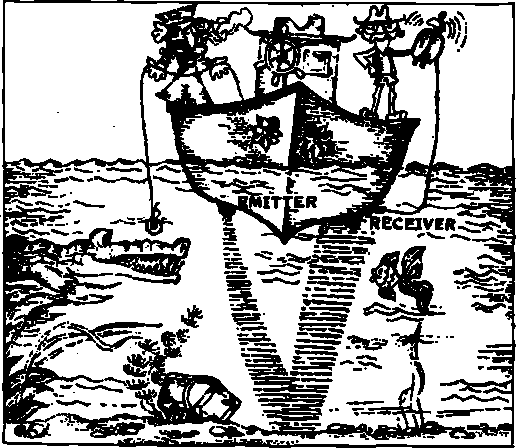
\includegraphics[width=0.9\textwidth]{figures/fig-06-13.pdf}
\caption{Using reflection of sound for measuring depth of a water body.}
\label{fig-6.13}
\end{figure}
The reflection of sound is widely applied in navigation. The construction of an instrument for measuring depths, the sonic depth finder, is based on it. A source of sound is placed under water on one side of a ship (\figr{fig-6.13}). A discontinuous sound creates sound rays, which will make their way through the watery thickness to the bottom of the sea or river, be reflected from the bottom and re­turn in part to the ship, where sensitive instruments will catch them. Accurate clocks will show how much time the sound needs for this journey. The speed of sound in water is known, and it is possible to obtain precise in­ formation about the depth by means of a simple calcula­tion.

By aiming the sound forward or sideways instead of downwards, it is possible to determine with its aid whether or not there are dangerous reefs or deeply submerged ice­ bergs near the ship.

All the particles of air surrounding a vibrating body are in a state of vibration. As we explained in the first book, a mass point vibrating in accordance with the si­nusoidal law possesses a definite and constant total energy.

When a vibrating point passes through its equilibrium position, its speed is maximum. Since the displacement of the point is equal to zero at this instant, the entire energy is kinetic:
\begin{equation*}%
E = \frac{mv^{2}_{\textrm{max}}}{2}
\end{equation*}
Consequently, the total energy is proportional to the square of the amplitude of the speed of vibration.

This is also true for particles of air vibrating in a sound wave. However, a particle of air is something indefinite. Therefore, sound energy is given per unit of volume. This magnitude can be called the density of sound energy.

Since the mass of a unit of volume is the density $\rho$, the density of sound energy
\begin{equation*}%
w = \frac{\rho v^{2}_{\textrm{max}}}{2}
\end{equation*}
Above we have spoken about another important phys­ical quantity which vibrates according to the sinusoidal law with the same frequency as the speed. This is the sound, or excess, pressure. Since these quantities are proportional, we can say that the energy density is pro­portional to the square of the amplitude of sound pressure.

The maximum value of the speed of sound vibration for loud conversation is equal to \SI{0.02}{\centi\meter\per\second}. One cubic cen­timetre of air weighs about \SI{0.001}{\gram}. Therefore, the energy density is equal to
\begin{equation*}%
\frac{1}{2} \times \num{d-3} \times \num{0.022}^{2} \si{\erg\per\centi\meter\cubed} = \SI{2d-7}{\erg\per\centi\meter\cubed}
\end{equation*}
Suppose that a source is emitting sound. It is radiating sound energy in the surrounding air. It is as though the energy were ``flowing'' from the vibrating body. During a second, a definite amount of energy flows through each area element, which is perpendicular to the direction of the propagation of the sound. This quantity is called the \emph{energy flux} passing through the area element. Furthermore, if we take an area element of \SI{1}{\centi\meter\squared}, the amount of energy which has passed through it is called the \emph{intensity of the sound wave}.

It is not difficult to see that the intensity $I$ of sound is equal to the product of the energy density $w$ by the speed of sound $c$. Imagine a small cylinder of \SI{1}{\centi\meter} height and \SI{1}{\centi\meter\squared} base area whose generatrices are parallel to the direction of propagation of a sound. The energy $w$ con­tained in such a cylinder will completely leave it during a time of $1/c$. Therefore, an energy of $w/(1/c)$, i.e. $wc$, will
pass through a unit of area during a unit of time. It is as though the energy were moving with the speed of sound.

During a loud conversation, the intensity of the sound near the talkers will be approximately equal to (we are making use of the number obtained above)
\begin{equation*}%
\num{2d-7} \times \num{3d4} = \SI{0.006}{\erg\per\centi\meter\squared\per\second} 
\end{equation*}

\section{Audible and Inaudible Pitches}

But what sounds can be perceived by the human ear? It turns out that the ear is capable of perceiving only the vibrations lying within the interval from approximately 20 to \SI{20000}{\hertz}. Sounds with a large frequency are called high-pitched, and those with a small frequency low-pitched.

But what wavelengths correspond to the limiting au­dible frequencies? Since the speed of sound is approximate­ly equal to \SI{300}{\meter\per\second}, using the formula $\lambda = cT = c/\nu$, we find that the lengths of audible pitches corresponding to wavelengths that lie within the limits of \SI{15}{\meter} for the lowest tones to \SI{3}{\centi\meter} for the highest ones.

And how do we ``hear'' these vibrations?

The way the organ of hearing functions has not as yet been fully clarified. The crux of the matter is that the internal ear (the cochlea, a canal of few centimetres long and filled with fluid) contains several thousand sensory nerves capable of perceiving sound vibrations transmitted to the cochlea from the air through the tympanic mem­brane. This or that part of the cochlea vibrates more strongly depending on the frequency of sound. Although the sen­sory nerves are situated along the cochlea so closely that a large number of them are stimulated simultaneously, man (and animals) is capable, particularly in childhood, of distinguishing minute changes in frequency (thousands of a fraction). It is still not known precisely just how this
occurs. The only obvious fact is that the analysis by the brain of the stimuli arriving from many different nerves is of utmost importance here. A mechanical model of the same design as the human ear that could be capable of discerning sound frequencies just as well has yet to be invented.

A sound frequency of \SI{20000}{\hertz} is the value beyond which the human ear does not perceive the mechanical vibrations of a medium. It is possible to create vibra­tions of a higher frequency in various ways; a person will not hear them, but instruments can record them. Inciden­tally, not only instruments record such vibrations. Many animals -- bats, bees, whales and dolphins (as can be seen, it isn’t a question of the dimensions of a living being) -- are capable of perceiving mechanical vibrations with frequencies up to \SI{100000}{\hertz}.

We are now able to obtain vibrations with frequencies up to a thousand million hertz. Such vibrations, although of inaudible pitch, are called \emph{ultrasonic} or \emph{supersonic} in order to affirm their affinity to sound. Supersounds of the highest frequencies are obtained with the aid of quartz plates. Such plates are cut out of monocrystals of quartz.